\begin{figure}
\centering
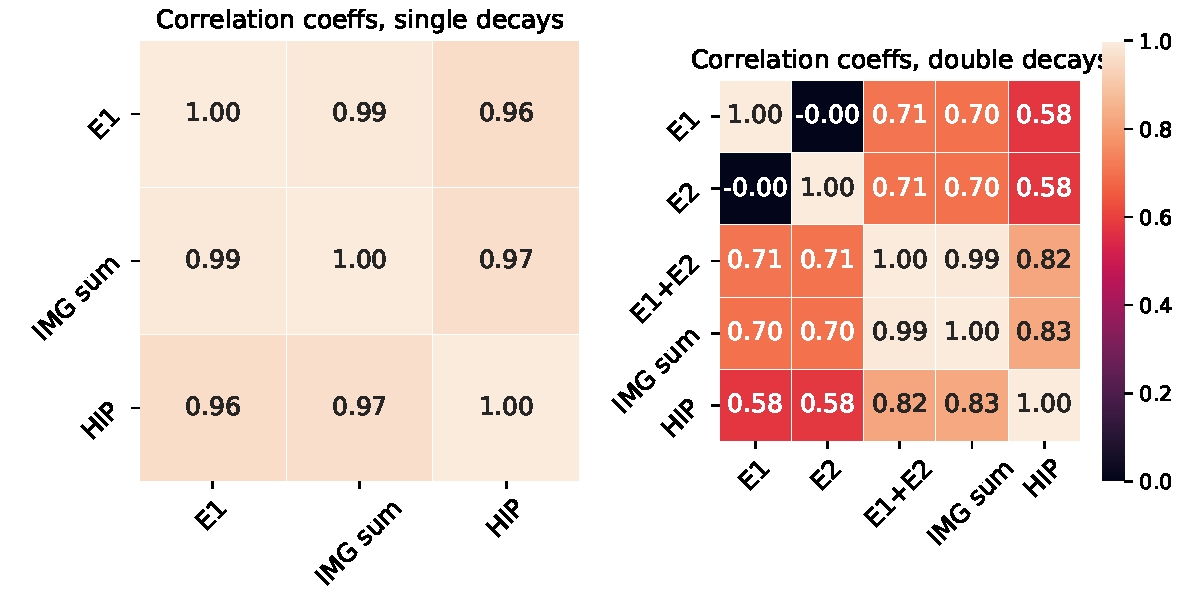
\includegraphics[width=\textwidth]{chapters/results/figures/simulated_corrcoeff.pdf}
\caption{\label{fig:simulated_corrcoeff}Correlation matrices for simulated data,
    separated into single and double decays. $E1$ and $E2$ are the energies corresponding
    to event 1 and event 2 in simulated data. For single events there is no event 2.
    $Sum(image)$ is the sum of all intensities per image in the dataset. HIP is short for
    Highest Intensity Pixel value.
    }
\end{figure}
